\section{Photovoltaic cells and Irradiance}\label{seq:pv_and_irradiance}

A photovoltaic (PV) cell is a component generating electricity from light by the photovoltaic effect. A PV-cell, illustrated in figure \ref{fig:pv-effect} consists of two semi-conductors, one with a surplus of electrons, the negative(N)-side, and one with a deficit, the positive (P)-side. Between the two semi-conductors is an electric field. Photons from sunlight energize the atoms on the N-side, freeing up an electron. This electron then travels through the circuit to the P-side, creating an electric current to be utilized by external loads.\\

\begin{figure}
    \centering
    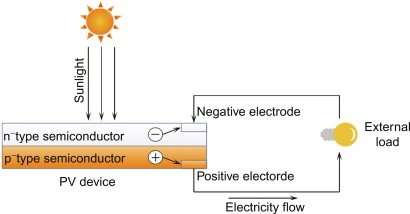
\includegraphics{Figures/06Design/pv_effect.jpg}
    \caption[PV-effect]{Illustration of the PV-effect. Figure from \textit{(Asdrubali, F. et al. 2019)} \cite{Asdrubali2019441}}
    \label{fig:pv-effect}
\end{figure}

The power produced by a PV-cell correlates with the power received from the sunlight.\cite{Frederick1995} The power per area is known as irradiance and is measured in $W/m^2$. There are different types of solar irradiance including
\begin{itemize}
    \item \textit{Global Tilted Irradiance(GTI)}    -   The total irradiance received on a surface with a given azimuth and slope.
    \item \textit{Direct Normal Irradiance(DNI)}    -   The irradiance measured on a surface element perpendicular to the sun's direction. Excludes irradiance scattered by the atmosphere. Dependent on weather and atmospheric conditions such as cloud cover.
    \item \textit{Diffused Horizontal Irradiance(DHI)}  -   The irradiance received on a surface element from light scattered by the atmosphere. Just as DNI, dependent on atmospheric conditions.
\end{itemize}

There are several methods for modelling the total irradiance(G) on a PV-panel given the GTI, DNI, DHI and weather conditions. In the paper \textit{(Frederick, J. E., and H. D. Steele, 1995)} the authors used the simple equation

\begin{equation}
    G = f*G_{DHI} + (1-f)*G_{GTI}
    \label{eq:irradiance}.
\end{equation}

Where $f$ is the cloud cover, $N_{DHI}$ the DHI and $N_{GTI}$ the GTI at the time of measurement. 

\section{Forecasting}
Forecasting is the process of making future predictions based on present or past information. Applied to microgrid control, this often means predicting the value of future demand and production. To be able to make accurate forecasts for these values is of crucial importance to effectively controlling the system. 

There are several different approaches to time-series forecasting. Amongst these are statistical and physical approaches. 

\subsection{Statistical approach}\label{seq:stat_forecasting}

\textit{Statistical forecasting} relies primarily on the historic values of a time-series to predict its future value. They assume an \textit{auto-regressive property}, meaning that a future value can partially be predicted based on past values.\\

A \textit{persistence model} is the most direct implementation of this assumption. It assumes that the current and historical conditions are similar  to some future ones. This is sometimes known as the naive approach and is mathematically expressed in equation \ref{eq:persistence}. The model can be  extended into an \textit{average model} by using the average over the past number of days to estimate the future value, as done in equation \ref{eq:persistence_avg}. For an average model, the key parameter to select is the \textit{look-back period}, meaning the amount of past terms to include in the calculation of the future value. In equation \ref{eq:persistence_avg} this is the \textit{k}-parameter. Additionally, a weighting of the different terms in the average model can be introduced to produce a \textit{weighted persistence model}. This, as shown in \ref{eq:weighted_persistence_avg}, will vary the impact of the different past terms for the final forecast. While allowing more flexibility, this is significantly more difficult to tune, as the weight vector will have equal length to the target vector. It is possible to simplify this by defining the weight as a function.    

\begin{equation}
    \hat{x}_{t+1} = x_{t}
    \label{eq:persistence}
\end{equation}

\begin{equation}
    \hat{x}_{t+1} = \frac{1}{(t-k)}\sum_{i=k}^{t}{x_t}     ,t>k>0
    \label{eq:persistence_avg}
\end{equation}

\begin{equation}
    \hat{x}_{t+1} = \frac{1}{(t-k)}\sum_{i=k}^{t}{w_i x_i}     ,t>k>0
    \label{eq:weighted_persistence_avg}
\end{equation}

An \textit{Auto-Regressive Integrated Moving Average (ARIMA) model} is a more complex statistical model and a commonly used framework for forecasting. It consists of an \textit{Auto-Regressive model} and a \textit{Moving-Average model}, with an integrated term. 

An auto-regressive model predicts the future value of a variable from the historical values of the variable. It is the same as the \textit{weighted persistence model} defined above. It is often denoted as AR(p) where p represents the order of the model i.e. how many past terms are included. Equation \ref{eq:ar_model} expresses this mathematically. 

A moving average model is most useful when a variable oscillates around some average $\mu$. It uses the average and the past deviation from the average to estimate the variable. Similar to an AR-model, a moving average model can have different orders and is denoted as MA(q) with a mathematical expression as seen in \ref{eq:ma_model}.

Lastly, the integrated term of the ARIMA is used if the original time-series expression has non-\textit{stationary} attributes. A stationary time-series has a time-invariant mean and variance. There are different kinds of stationarity, such as \textit{wide-sense stationarity}, which allows for cyclic behaviour within a time-series as long as the series is stationary across the period. Both the AR- and the MA model require a stationary time-series to perform optimally. If the time-series itself is not stationary, meaning that the mean or variance is time-variant, a differentiated time-series with values expressed by equation \ref{eq:differencing} for either a 1. or 2. order difference can be utilised to remove the non-stationary components. The order of the differentiating term can be written as I(d). Together with the AR and MA model, an ARIMA model of order p,d and q can be written as ARIMA(p,d,q).
\begin{equation}
    x_t = \sum_{i=1}^{p}{\phi_i x_{t-i}} + \epsilon_t
    \label{eq:ar_model}
\end{equation}

\begin{equation}
    x_t = \mu + \sum_{i=1}^{q}{\theta_i \epsilon_{t-i}} + \epsilon_t
    \label{eq:ma_model}
\end{equation}

\begin{align}
    x_t' &= x_t - x_{t-1}        (1.order)\notag\\
    x_t^* &= x_t' - x_{t-1}'     (2.order)
    \label{eq:differencing}
\end{align}

An ARIMA can be extended to account for seasonal components of a time-series. Such a model is known as a seasonal ARIMA (\textit{SARIMA}) model. In addition p,d and q coefficients, the SARIMA has the additional P, D, Q and a seasonality constant. Similarly to the coefficients for the regular  ARIMA, these coefficients define how many terms are to be included for the AR, I and MA models respectively, only that they are shifted backwards by the seasonality constant. 

\subsubsection{Model and parameter selection ARIMA}\label{seq:tuning_arima}
There are several methods for choosing the appropriate model and parameters for an ARIMA model, one of the most common is the \textit{Box-Jenkings method}. The Box-Jenkings method is a step-wise algorithm for choosing the best fit ARIMA-model. The first step is model identification and selection. This means finding the correct values for the ARIMA-parameters \textit{p,d,q,P,D,Q and s}. A prerequisite for selecting these parameters is to examine the seasonal and stationary behaviour of the time-series.\\ 

The seasonal behaviour is often known a priori, but if not it can be inferred through an ACF plot by examining the terms within a confidence interval. It is the length of the period over which the pattern repeats itself. In our systems, we know in advance that both demand and production follow a daily cyclic pattern. This yields the seasonal parameter \textit{s}.\\

Both the AR- and MA-model perform sub-optimally if the time-series exhibits strong non-stationary behavior.  If a series is wide-sense stationary, an ARMA model is in theory sufficient for forecasting. Stationarity can be determined from a time-series plot, but there are also tests developed. One of the test for stationarity is the \textit{Augmented Dicker-Fuller}-test (ADF-test).\\ 

The ADF-test test the null hypothesis that the unit root is part of the process' characteristic equation. If the null hypothesis is accepted, it means that the unit root is present, and the process is non-stationary. On the other hand, the null hypothesis might be rejected. The test statistic $\mathbf{DF}$ obtained from the test indicates how strongly the null hypothesis is rejected. If this is more negative than some critical value, it indicates that the process is stationary. The result of this process is the order of differentiating, the \textit{d}-term. A key point regarding differentiating is although it can achieve better stationarity, it may remove some of the information from the time-series.\\

When the stationary and seasonal behaviour of the process is determined, then the order of the AR and MA models can be obtained from the partial auto-correlation function (PACF) and auto-correlation function respectively.\cite{Zuleta-Elles2021-qh}\\

The order of the auto-regressive model can be found in the partial auto-correlation function. The PACF gives the direct correlation between a past term $x_{t-k}$ and the target term $x_t$ removing any indirect effect through intermediate terms $x_{t-1},..., x_{t-k+1}$. The order of the AR model only includes terms with a statistically significant direct effect on the target term. Its connection to the PACF is therefore intuitive as the PACF will only show terms above a confidence interval if they have a statistically significant effect on the target term. Hence its order is equal to the amount of terms of the PACF before the PACF goes outside the confidence interval. This will yield the \textit{p}-term of the ARIMA-model.\\
%\todo{Show plots?}

The order of the moving average model, on the other hand, can be determined from the auto-correlation function. The ACF gives the correlation between a past term $x_{t-k}$ and the target term $x_t$, including both the direct effect and the indirect effect through intermediate terms. The connection between the ACF and the order of the MA-model is less intuitive than that between the PACF and AR-model. The following is an attempt to connect the two based on the method in \cite{Ritvikmath2019-np}:\\

Consider a MA(q) model as described by equation \ref{eq:ma_model}. Expanded, this will look like
\begin{equation}
    MA(q): x_t = \mu + \theta_{t-1} \epsilon_{t-1} + ... + \theta_{t-q} \epsilon_{t-q} + \epsilon_t
    \label{eq:ma_model_expanded}.
\end{equation}

The ACF gives the correlation between the target term and past terms. The correlation between $x_t$ and $x_{t-l}$ can be written as

\begin{equation}
    Corr[x_t,x_{t-k}]   =   \frac{Cov[x_t,x_{t-k}]}{\sigma_{x_t}\sigma_{x_{t-k}}}
    \label{eq:ma_corr}.
\end{equation}

Assuming a non-zero variance, the denominator of \ref{eq:ma_corr} will be some constant. For selecting the order of the MA-model, we are interested in when the ACF is zero. The denominator can therefore be neglected, and we are left with a proportional equation as

\begin{equation}
    Cov[x_t,x_{t-k}]    =   E[x_t x_{t-k}] - E[x_t] E[x_{t-k}]
    \label{eq:ma_cov}.
\end{equation}

The $E[x_t]$-term can be expanded as

\begin{align}
    E[x_t] & = E[\mu + \theta_{t-1} \epsilon_{t-1} + \ldots + \theta_{t-q} \epsilon_{t-q} + \epsilon_t ] \notag \\
           & = E[\mu] + \theta_{t-1} E[\epsilon_{t-1}] + \ldots + \theta_{t-q} E[\epsilon_{t-q}] + E[\epsilon_t]
    \notag \\
           & = \mu + \theta_{t-1} E[\epsilon_{t-1}] + \ldots + \theta_{t-q} E[\epsilon_{t-q}] + E[\epsilon_t].
\end{align}

As the error of a stationary process is assumed to be unbiased, every term involving $E[\epsilon]$ is therefore equal to zero. We are left with

\begin{equation}
    E[x_t] = \mu.
\end{equation}

Equation \ref{eq:ma_cov} can therefor be written as 

\begin{equation}
    Cov[x_t,x_{t-k}]    =   E[x_t x_{t-k}] - \mu^2
    \label{eq:cov_semi}.
\end{equation}

The $E[x_t x_{t-k}]$ is more complicated. Using the definition in \ref{eq:ma_model_expanded}, the product $x_t x_{t-k}$ can be written as 

\begin{align}
    x_t x_{t-k} &= (\mu +\theta_{t-1} x_{t-1} +...+\theta_{t-q}x_{t-q})(\mu +\theta_{t-k} x_{t-k} +...+\theta_{t-k-q}x_{t-k-q})\notag \\
    &= \mu^2 + \mu(\theta_{t-k} x_{t-k} +...+\theta_{t-k-q}x_{t-k-q})\notag\\
    &+\theta_{t-1}x_{t-1}(\mu+\theta_{t-k} x_{t-k} +...+\theta_{t-k-q}x_{t-k-q})+...\notag\\
    &+\theta_{t-q-1}x_{t-q-1}(\mu+\theta_{t-k} x_{t-k} +...+\theta_{t-k-q}x_{t-k-q})
    \label{eq:cov_product}.
\end{align}

The $\mu^2$ from \ref{eq:cov_semi} and \ref{eq:cov_product} will cancel each other out. From equation \ref{eq:cov_product} we are then left with three kinds of terms when inserted into \ref{eq:cov_semi}: Either 
\begin{align}
    I: & \mu \theta_{t-r}E[x_{t-r}], r=1,2...q\notag\\
    II:& \theta_{t-r}\theta_{t-l}E[x_{t-r}x_{t-l}], l\neq r\notag\\
    III:& \theta_{t-r}^2E[x_{t-r}^2].
\end{align}

Because the errors are independent of each other and unbiased, terms $I$ and $II$ are equal to zero. The only terms that will not be equal to zero is the $III$ terms, because that would imply zero variance. These terms will only appear if $x_t$ and $x_{t-k}$ have overlapping terms. Going back to \ref{eq:cov_semi} we have that

\begin{align}
    Cov[x_t,x_{t-k}] \neq 0 \iff t-q\leq t-k \implies k\leq q.
\end{align}

This then means that from the ACF, the only way to get a non-zero value is if the term is less than or equal to the order of the MA-model. Hence the \textit{q} from the MA-model may be determined from the ACF.

The terms for the seasonal component \textit{P,D and Q} can by determined through the same process as for the non-seasonal, but looking at the behaviour one period back. The ACF and PACF will often have a spike at a lag of one period, this may then be included as the order of the seasonal model. If the model is trending between seasons, a seasonal differtiating term of order \textit{D} may be included.


\subsection{Physical approach}\label{seq:physical_forecasting}
\textit{Physical models} on the other hand are built on the physics of the system. The forecast is therefore based on the system dynamics and external input. In this thesis, a physical model is used to predict power production from the solar panels based on solar irradiance. Therefore, an outline of the relationship between solar irradiance and power is included here.\\

Irradiance is measured in power over area $(W/m^2)$. The irradiance cast onto the panels depends on the location, orientation and angle of the panels, in addition to the weather conditions. The amount of the irradiance that is converted to electrical power is dependent on total panel size and efficiency, this is given by \ref{eq:pv_power_simple}. The efficiency $\eta$ is often found during the testing of the panels. It is expressed in \ref{eq:pv_efficency} where $P_{STC}$ and $G_{STC}$ represent the power and irradiance under \textit{standard testing conditions} (STC) respectively. Together, that gives the complete equation for the power given by each panel seen in \ref{eq:pv_power_full}. 

\begin{equation}
    P = \eta A G
    \label{eq:pv_power_simple}
\end{equation}

\begin{equation}
    \eta =  \frac{P_{STC}}{A G_{STC}}
    \label{eq:pv_efficency}
\end{equation}

\begin{equation}
    P = \frac{P_{STC}}{G_{STC}} G
    \label{eq:pv_power_full}
\end{equation}


Specifically for the case considered in this thesis, we want to obtain a predicted time-series of the production for some time into the future. 

\subsection{Error metrics for forecasting}
It is crucial to be able to evaluate a forecast, to assess the suitability of a forecaster. This is in general done by comparing the forecasted time-series $F$ to the actual time-series $A$. The measurement error $\varepsilon_i$ at time-step $i$ is defined in equation \ref{eq:measurement_error}. One could find the error for all measurements and combine them into a vector. This will yield an error vector equal in size to the $A$ and $F$. It is common to reduce the errors for all samples into a single error statistic. The most common of these are \textit{Root Mean Square Error} (RMSE), \textit{Mean Average Error} (MAE) and \textit{Mean Average Percentage Error} (MAPE). The difference between these in their intuition and accuracy requires an informed decision about the choice of error metrics.

\begin{equation}
    \varepsilon_i = A_i - F_i
    \label{eq:measurement_error}
\end{equation}

MAPE, shown in equation \ref{eq:mape}, is perhaps the most intuitive, as the percentage error will follow the scale of the measurements. It has however a few major drawbacks.\cite{MAKRIDAKIS1993527} As discussed in \textit{(Makridakis, S., 1993)}, MAPE is poorly suited to compare different models as it will systematically bias towards forecasts lower than the actual time-series. This is because it punishes over-estimates harsher than under-estimates. Consider a situation with an actual timeseries $A$ and a forecasted series $F$ with $A_1 = 1$, $A_2 = 3$ and $F_1 = F_2 = 2$. The absolute percentage error between $A_1$ and $F_1$ is $\frac{|A_1-F_1|}{A_1}*100\%=100\%$, between $A_2$ and $F_2$ however it is $\frac{|A_2-F_2|}{A_2}*100\%=33.3\%$\cite{kolassa2011}. This shows that the same absolute deviance from the actual time-series receives a higher MAPE if the forecast is above, than if it is below the actual value. There have been efforts to avoid this bias, however then at the loss of the intuitive appeal of the method.\\

Both RMSE and MAE, shown in equation \ref{eq:rmse} and \ref{eq:mae} respectively are better suited because they avoid this bias. These methods are fairly similar to each other, however, the MAE has some advantages making it more appropriate. First of all, it is arguably more intuitive than the RMSE. Secondly, it varies proportionally with the absolute error, while the RMSE does not as it also varies with the root of the number of errors\cite{Willmott2005-go}.

\begin{equation}
    \text{RMSE} = \sqrt{\frac{1}{n} \sum_{i=1}^{n} (\varepsilon_i)^2}
    \label{eq:rmse}
\end{equation}

\begin{equation}
    \text{MAE} = \frac{1}{n} \sum_{i=1}^{n} |\varepsilon_i|
    \label{eq:mae}
\end{equation}

\begin{equation}
    \text{MAPE} = \frac{1}{n} \sum_{i=1}^{n} \left|\frac{\varepsilon_i}{A_i}\right| \times 100
    \label{eq:mape}
\end{equation}




\section{Reliability and System Sizing}\label{sec:reliability}
Reliability describes the ability of a system to function under stated conditions. There are several methods for measuring reliability over some period of time, amongst these are:
\begin{itemize}
    \item \textit{System Average Interruption Frequency Index} (SAIFI)    -   The average number of interruptions that occurred per system.
    \item \textit{System Average Interruption Duration Index} (SAIDI)    -   The length of interruptions per system.
    \item \textit{Average Service Availability Index} (ASAI)    -   The average unavailability of supply from a system, or parts of a system, compared to the total demand. 
\end{itemize}

If the loads are stratified based on priority, the reliability can be subdivided into reliability for types of loads such as critical reliability for critical loads, non-critical reliability for non-critical loads and total reliability for all loads. In microgrid systems, the reliability is dependent on the relationship between energy production, storage and consumption. In \textit{(Mehra, V. et al., 2018)} the reliability of a PV-microgrid system is described by a function of installed PV and Battery capacity visualised as in Figure \ref{fig:mehra_reliability_full} where the function values are found through simulation.\cite{Mehra2018-xs}. 

Such a function allows for a structured approach to system sizing, for instance through optimization. The authors in \textit{(Mehra, V. et al., 2018)} propose an optimization formulation minimizing the installation cost while preserving reliability above a certain threshold. The optimization problem is shown in equation \ref{eq:size_minimization} where $c, c_{k}$ and $c_{l}$ are the total cost, cost of Battery capacity and PV-capacity respectively. $B$ is the battery capacity while $PV$ is the $PV$ is the PV-capacity. The $TR$ represents the total reliability and the $CR$ the critical load reliability, here set to be no less than 90\% and 99\% respectively.\textit{(Mehra, V. et al., 2018, p.81)}\cite{Mehra2018-xs}

\begin{figure}[h]
    \centering
    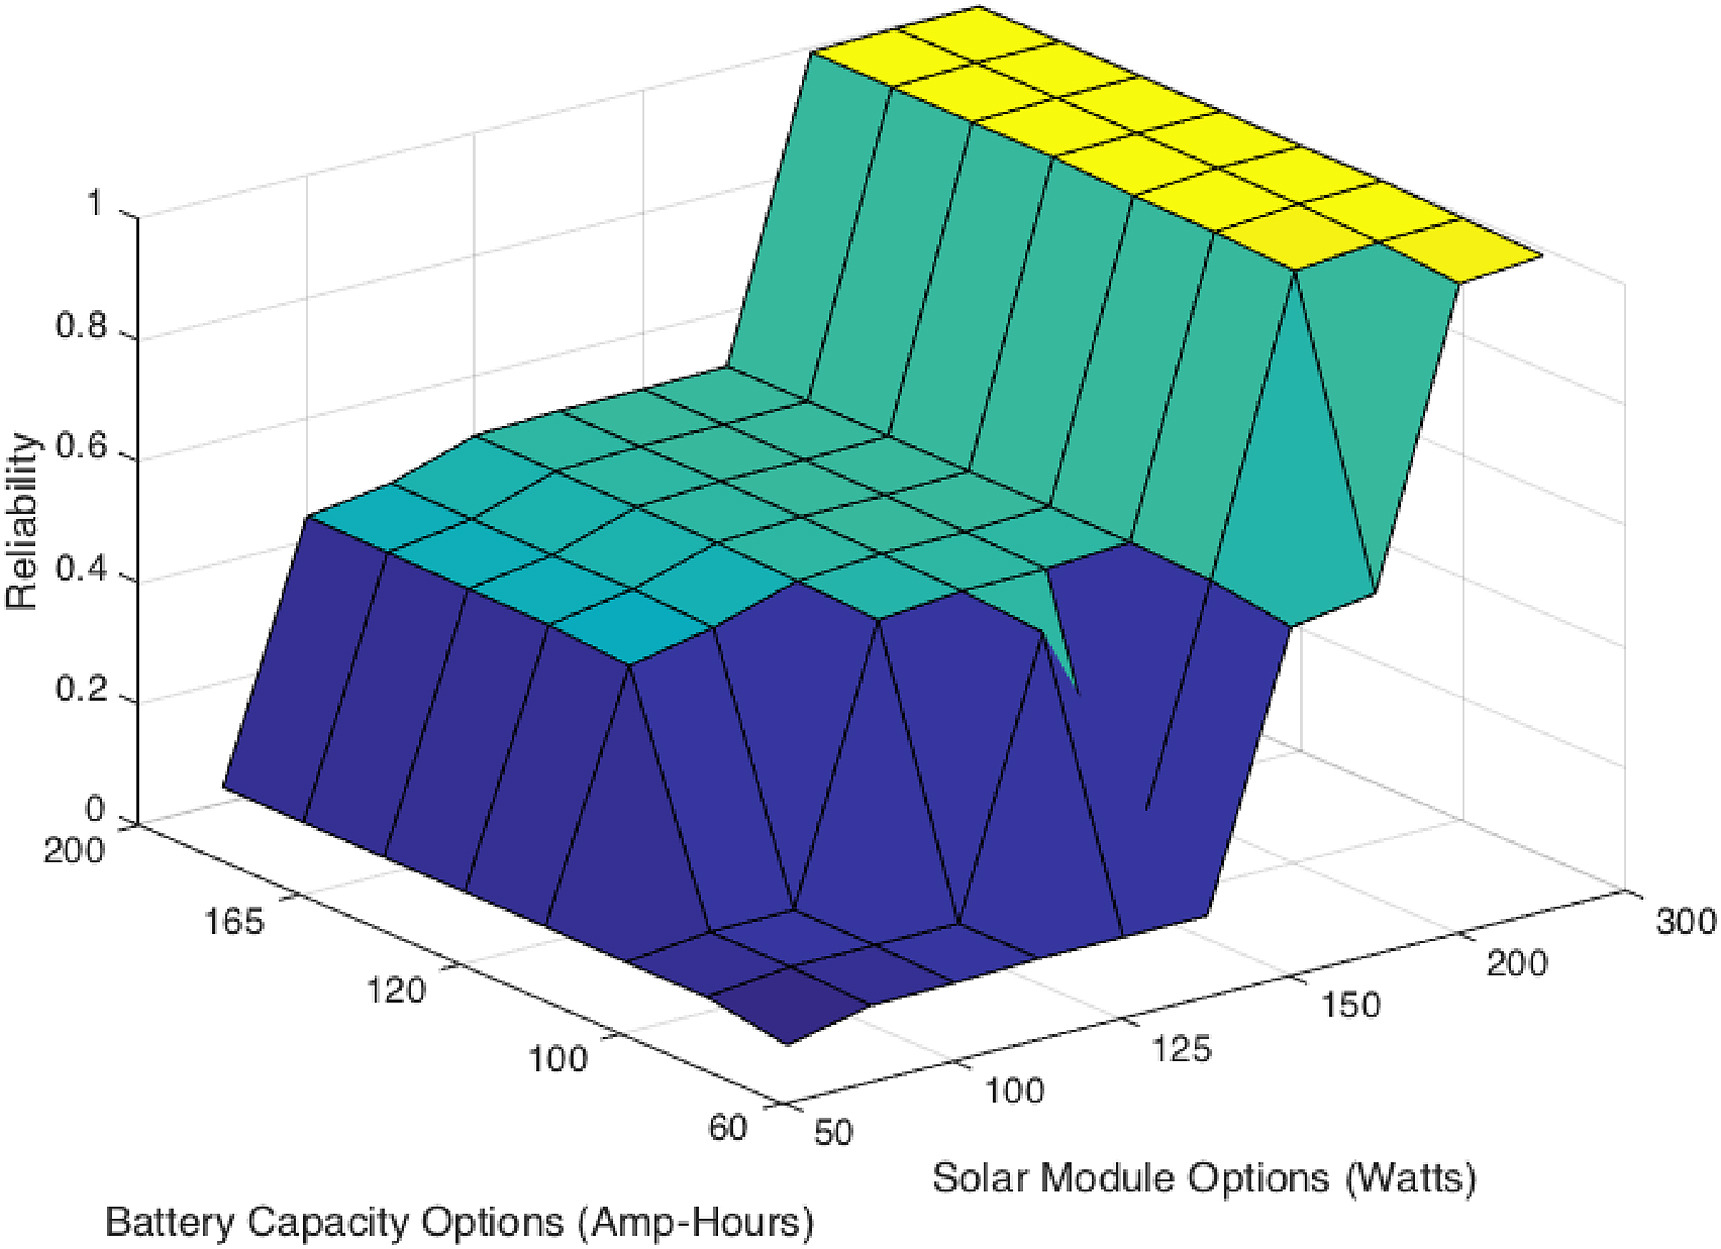
\includegraphics[width=\textwidth]{Figures/05Theory/mehra_reliability_full.jpg}
    \caption[Critical Load Reliability Plot]{Critical load reliability plot from \textit{(Mehra, V. et al., 2018 p.82)}\cite{Mehra2018-xs}. Reliability is expressed here as a function of PV and Battery Capacity, taking values from 0 to 1.}
    \label{fig:mehra_reliability_full}
\end{figure}

\begin{align}
    \min_c\hspace{0.5cm} & c = c_k * B + c_l * PV\notag\\
    \text{s.t.  } & TR \geq 90\%\notag\\
    & CR \geq 99\%
    \label{eq:size_minimization}
\end{align}


\section{Battery Health}\label{seq:battery_health}

Batteries are complex electrochemical components storing energy. The total charge of a battery is described in \ref{eq:battery_lifetime} as how low one can drain the battery, i.e. \textit{Depth of Discharge (DOD)}, multiplied by the number of cycles a battery is expected to last. Batteries are therefore components with a natural lifetime, which will gradually decline with usage. There are however additional effects that may accelerate the deterioration more rapidly than the natural usage. As batteries are amongst the most expensive equipment of a microgrid, it is of great value to control the microgrid in such a way as to not decrease the expected lifetime beyond its natural degradation. \\

\begin{equation}
    E_{tot} = DOD * n_{cycles}
    \label{eq:battery_lifetime}
\end{equation}

Two terms important for understanding batteries are
\begin{itemize}
    \item \textbf{State of Charge (SOC)}    -   SOC is a number usually represented by a percentage from 0-100\%. It shows how much capacity remains in the battery as a portion of its capacity at full state of charge.
    \item \textbf{Charge/Discharge-rate (C-rate)}    -   The power passed to/from a battery is dependent on the battery voltage and the current passed or drained to/from the battery. As voltage should remain relatively stable, the charge/discharge current specifies the charge/discharge rate. The discharge current is often normalised against the battery capacity using C-rate.\cite{MIT_Electric_Vehicle_Team2008-vm}. "The C-rate is a measure of the rate at which a  battery is discharged relative to its maximum capacity" \textit{(MIT Electric Vehicle Team, 2008, p.1)}\cite{MIT_Electric_Vehicle_Team2008-vm}  For instance, a battery of capacity 10Ah will have a C-rate of 1 if 10Amps is being discharged. If 5Amps is being discharged, then the C-rate would be 0.5C. A fully charged battery discharging at 0.2C would be fully discharged within 5 hours. The battery voltage of the batteries in this thesis is stable. Hence the C-rate will be used interchangeably with the rate of power charged/discharged from the battery.
\end{itemize}



The effects leading to  battery deterioration, or ageing, can be broadly classified as relating to either 
\begin{itemize}
    \item \textit{Calendar ageing}  -   The deterioration occurring under \textit{potentiostatic} hold, i.e. when low to no current is passing through the batteries. These effects are independent of the cycling behavior of the batteries, but influenced by factors such as the State of Charge and temperature during the potentiostatic hold. 
    \item \textit{Cycle ageing}  -   The deterioration inflicted during the active usage of the batteries. Depends on the Depth of Discharge, charge/discharge-rate. These effects may be further influenced by external factors such as temperature. 
\end{itemize}

In two papers, \textit{(E. Sarasketa-Zabala et al., 2014)} and \textit{(M. Naumann et al.,2018)}, lithium-ion batteries were stored under different combinations of temperature and SOC. In an experimental setup with several batteries at constant temperatures but different SOCs, their findings implied a stronger decrease in battery capacity for the  batteries stored at a high SOC. \cite{NAUMANN2018153} In \ref{fig:battery_calendar_aging} the experimental results from \textit{(E. Sarasketa-Zabala et al., 2014)} plotted. As a function of time, the plot shows that the capacity loss is greater when the battery is stored at a high SOC compared to other batteries at the same temperature.\cite{SARASKETAZABALA201445}  This indicates that calendar ageing can be reduced by reducing the time a battery spends at a high SOC.\\

\begin{figure}
    \centering
    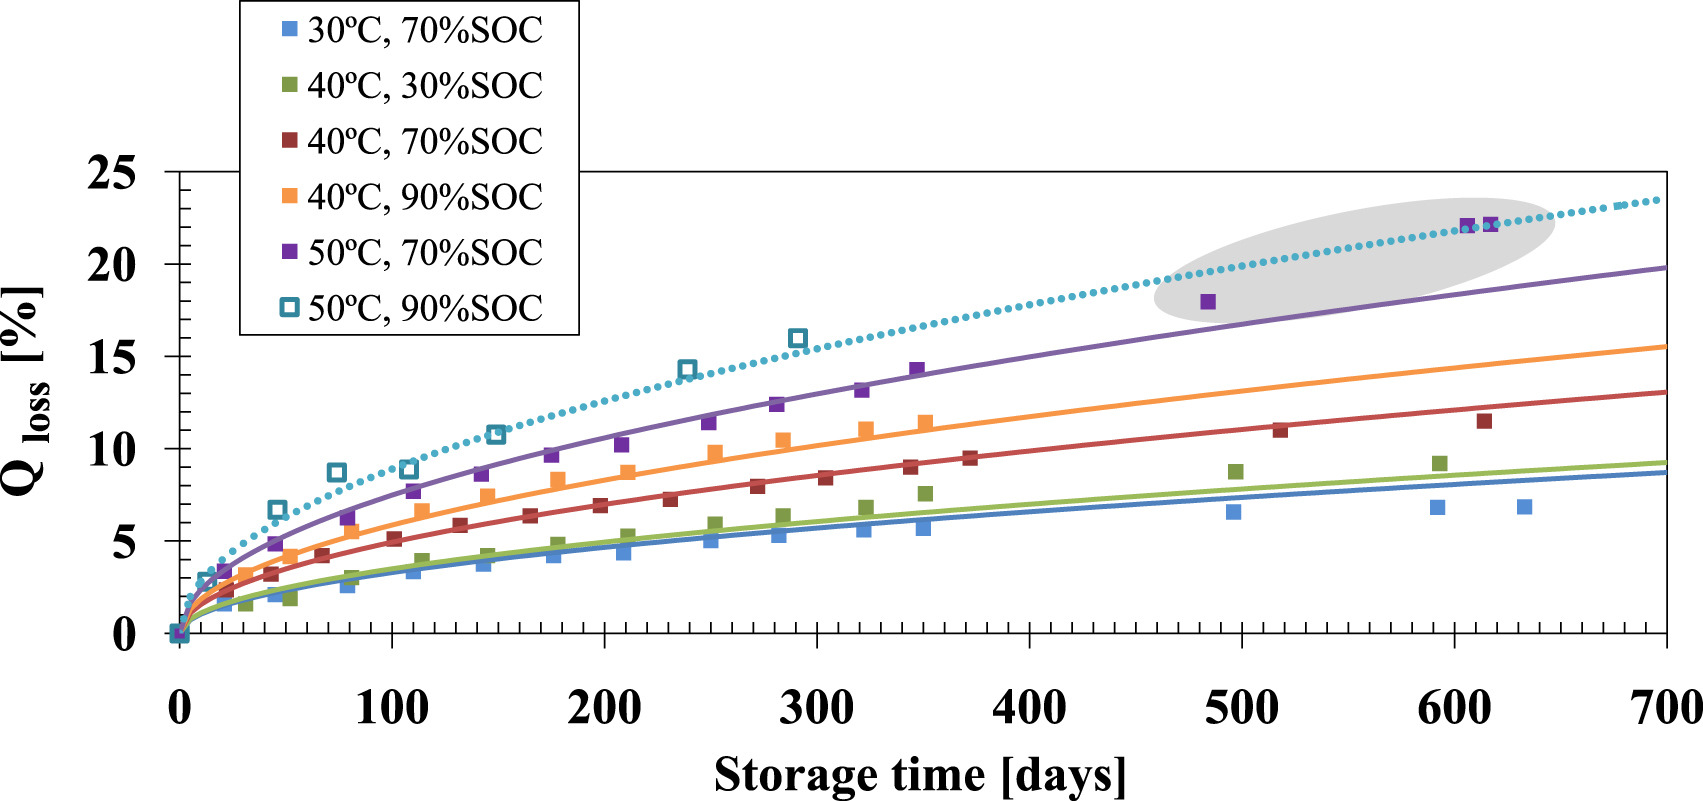
\includegraphics[width=\textwidth]{Figures/05Theory/battery_calendar_aging.jpg}
    \caption[Battery Calendar Aging]{Battery Calendar Aging from \textit{(E. Sarasketa-Zabala et al., 2014 p.53)}\cite{SARASKETAZABALA201445}. The y-axis shows the capacity loss $\mathbf{Q_{loss}}$ as a percentage of the battery capacity.}
    \label{fig:battery_calendar_aging}
\end{figure}

\begin{figure}
    \centering
    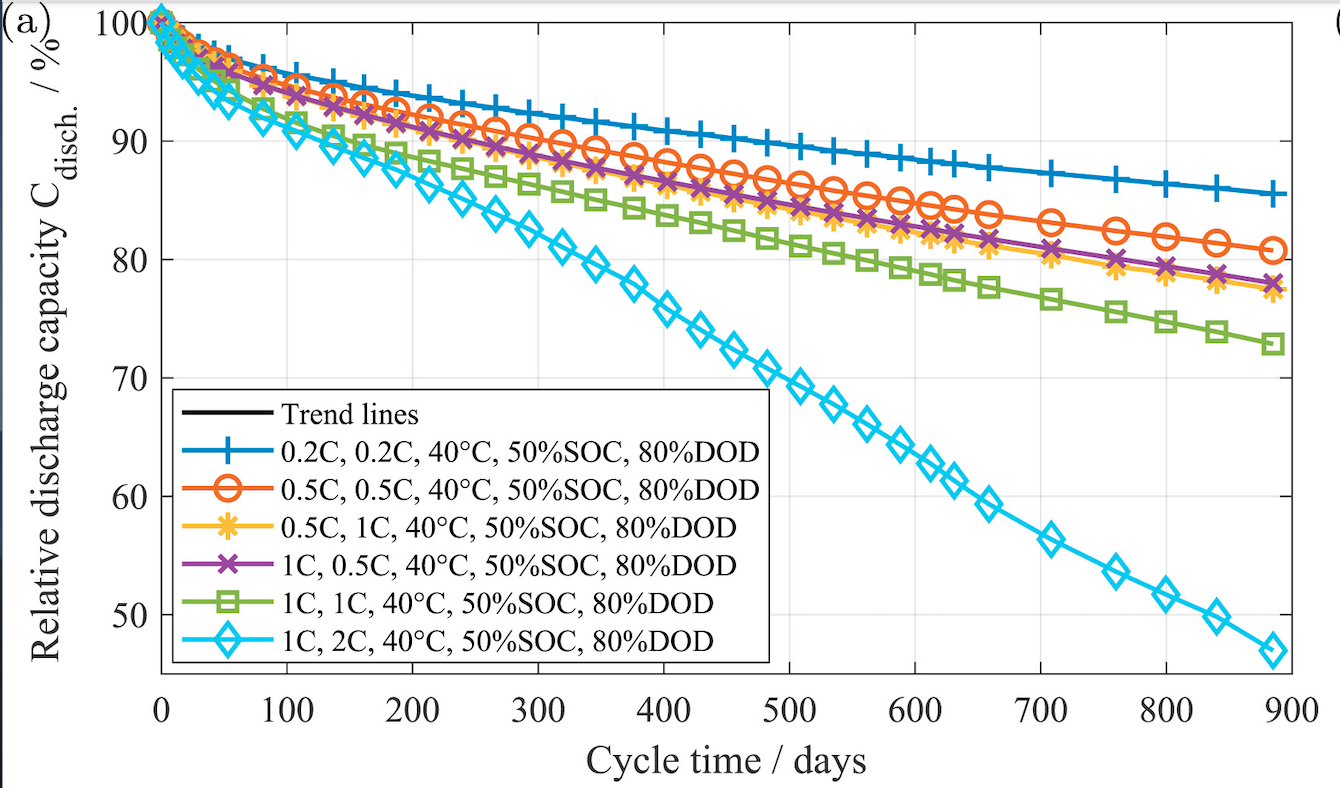
\includegraphics[width=\textwidth]{Figures/05Theory/battery_cycle_aging_cut.png}
    \caption[Battery Cycle Aging]{Battery Cycle Aging from \textit{(M. Naumann et al.,2020 p.6)}\cite{NAUMANN2020227666}.The y-axis shows the relative discharge capacity $\mathbf{C_{disch}}$.}
    \label{fig:battery_cycle_aging_cut}
\end{figure}

The same authors later published two papers considering cycle ageing. In a similar setup, lithium-ion batteries were cycled at different DOD, charge/discharge rates around different SOC points. All under varying temperatures. The results, where the ones from \textit{(M. Naumann et al.,2020)} is shown in \ref{fig:battery_cycle_aging_cut} show that the time-wise decrease in the discharge capacity is greater at high charge/discharge rates when the other conditions are kept equal. The best result in terms of time-wise degradation was in their results at 0.2C.\cite{SARASKETAZABALA2015573}\cite{NAUMANN2020227666}. 

The studies into battery cycle and calendar ageing therefore suggest that the control system should aim to 
\begin{itemize}
    \item \textit{Keep charge/discharge low}    -   Limit the current in and out of the battery to limit cycle ageing. Preferably at no higher than 0.2C.
    \item \textit{Avoid potentiostatic hold at high SOC}    -   When the battery is not used, it should not rest at a high SOC because of the effect on calendar ageing. 
\end{itemize}